\section{Solution Overview \& Main Techniques}
\label{sec:approach}

In this section, we present an overview of our solution: \name that on the high-level, uses the concept of the \emph{bump in the wire} (such as bump in the ether~\cite{McCPerRei2006}) to provide integrity and confidentiality to the user IO{}s between the IO devices and the remote server. \name achieves this by utilizing a trusted embedded device as a mediator between all the IO devices and the untrusted host. Hence, our approach fall into the category \textbf{B1} (external HW) in Figure~\ref{fig:relatedWorksTree}. We call this trusted intermediary \device for the rest of this paper.   %The server also adds a small JavaScript snippet that allows the \device and the remote server to communicate. This eliminates any need for additional hardware/software aids.

We first define the system and attacker model, then outline the challenges and the brief outline of our proposed solution.

%Given the problem statement discussed in Section~\ref{sec:problemStatement}, we first define the attacker model we consider in our proposed system.


\subsection{System Model}
\label{sec:approach:systemAttackerModel}


\begin{figure}[t]
\centering
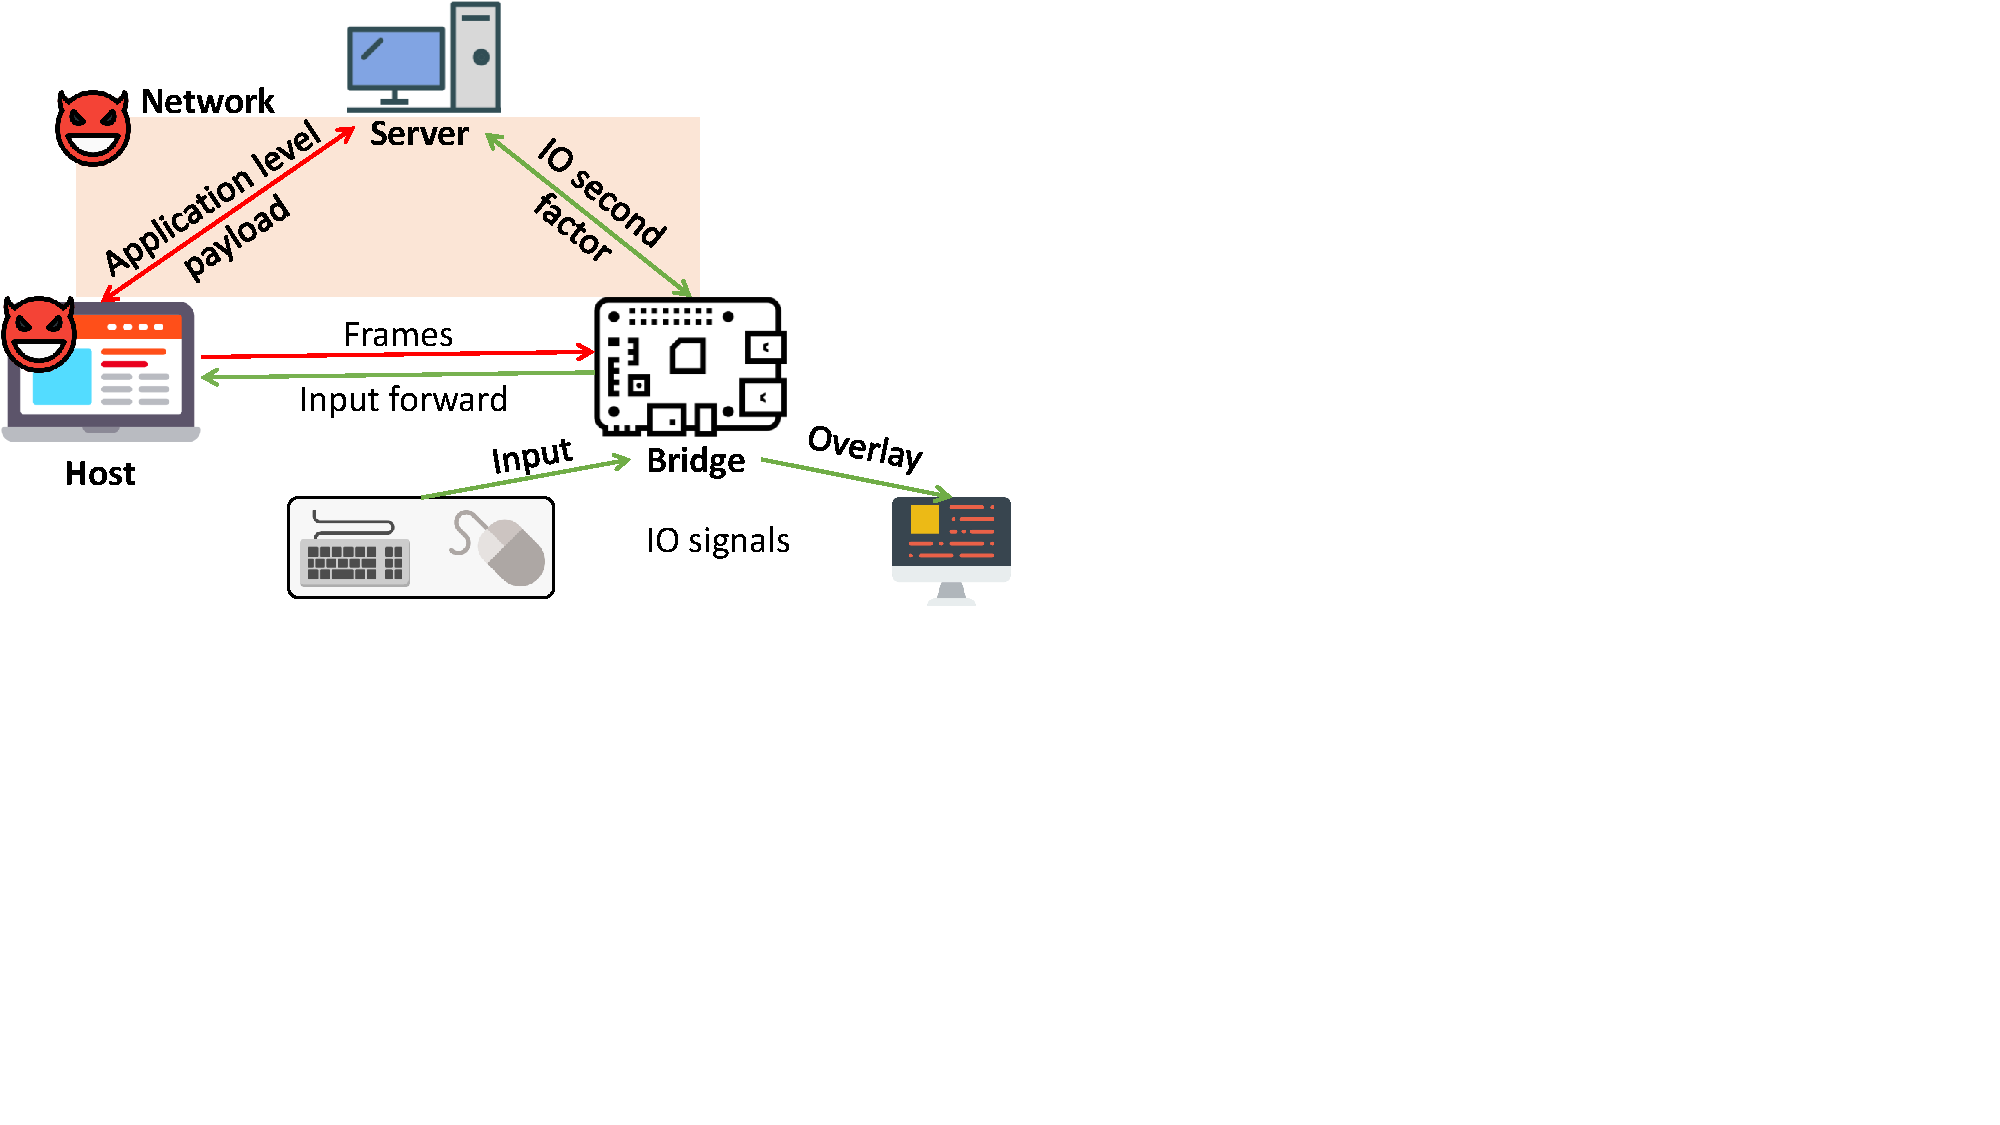
\includegraphics[trim={0 8.5cm 17cm 0}, clip, width=0.85\linewidth]{approachOverview.pdf}
\caption{\textbf{High-level approach overview of our solution.}  The \device connects the IO devices and the attacker-controlled host. We also assume that the network is also attacker-controlled.}
\spacesave
\label{fig:approachOverview}
\centering
\end{figure}


We consider a system model where the user wants to sends the input to a safety-critical remote end-system. The model is depicted in Figure~\ref{fig:approachOverview} that shows the untrusted host, remote server and the user IO devices. 
We only assume that the monitor, keyboard, mouse (in a word all the IO devices that we need to protect from the malicious host) and the \device are trusted.


The \device works as a mediator between all the IO devices and the host. Note that the \device has no network capability to communicate with the server, rather it relies on the host and uses it as an untrusted transport. We also assume that the \device comes with some embedded certificates and keys that allow the \device to verify the signatures signed by the server and sign statements such as the user input. We can assume that the \device is issued by a service provider who also runs the remote server.


\iffalse
\begin{figure}[t]
\centering
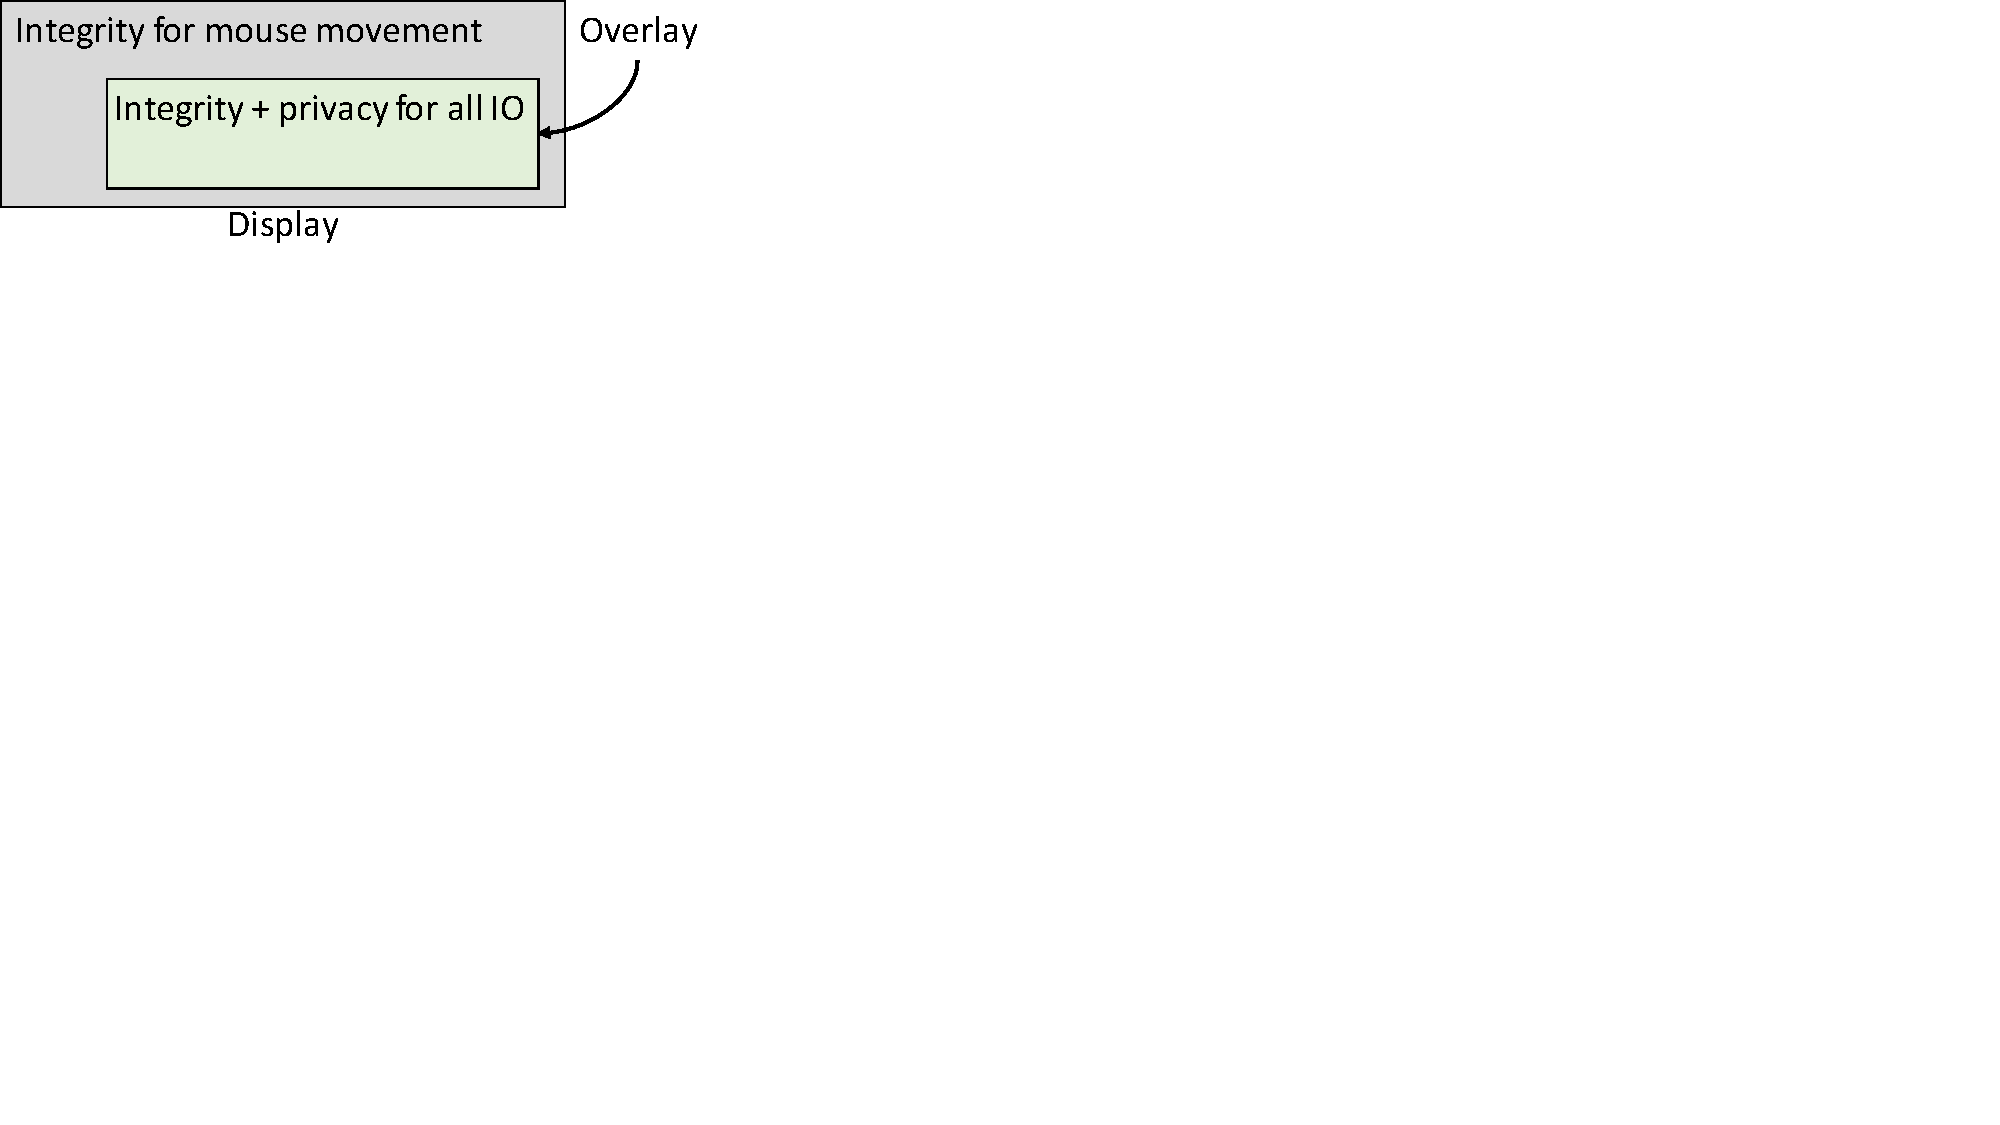
\includegraphics[trim={0 13cm 21.7cm 0}, clip, width=0.65\linewidth]{screenPartition.pdf}
\caption{\textbf{\device's pointer tracking, pointer \& UI overlay, and security properties.} Our proposed method provides two layers of protection for IO to the user. 1. In all the parts of the screen, the \device provide pointer integrity (the gray part). 2. The green part of the screen where the \device overlays on the HDMI stream where the \device provide integrity and privacy (privacy is dependent on the application requirements) for the IO.}
\spacesave
\label{fig:screenPartition}
\centering
\end{figure}
\fi

\iffalse
\subsection{Strawman Solutions}
\label{sec:approach:strawman}

Here we provide three strawman solutions and discuss the major drawbacks of such a solution.

\subsubsection{\bfseries Full-fledged isolated system}
\label{sec:approach:strawman:1}

The first strawman solution uses an external trusted device that runs a full operating system with a browser and is physically isolated from the attacker-controlled host. From the security point of view, this solution does not provide any security benefits - the external device as the same attack surface as the untrusted host due to its huge TCB, making it as vulnerable as the host.

\subsubsection{\bfseries Signing of input parameters}
\label{sec:approach:strawman:2}

The second strawman solution uses the concept of bump-in-the-wire, i.e., a trusted external device that contains a small program that signs all the user input and sends the signed input to the remote server. The device works as the second factor for input integrity as the remote server can verify if the signed input matched with the user input that is sent by the browser running on the untrusted host. IntegriKey~\cite{IntegriKey} provides such a solution that uses \webusb to send the signed input to the remote server. However, as the external device is completely oblivious to the display information that the untrusted host renders, it is vulnerable to a sophisticated UI manipulation attack. E.g., assume that the user's correct input is $100$. However, the host shows her $10$ on the text field. Thinking that she may have mistyped, the user types another $0$ that makes the recorded input from the user $1000$. This attack violates input integrity as the host can now submit $1000$ to the remote server as the external trusted device also signs $1000$ as the correct input received from the user.  


% \subsubsection{\bfseries Strawman solution III}
% \label{sec:approach:strawman:3}
% 
% This strawman solution is identical to Fidelius~\cite{Fidelius} where an external device sits between all the IO device and overlays on the textbox to achieve input confidentiality. As the device does not look into the output on the screen, the attacker can always manipulate the UI (such as changing the unit of the input or add some malicious instruction) to compromise the integrity of the user input data. On top of that, as the UI objects apart from the textboxes are not protected, the malicious OS can always emulate mouse events, e.g., submit the data to the remote server before the user finishes her input. 

\subsubsection{\bfseries Capturing screenshot}
\label{sec:approach:strawman:3}

\iffalse
\begin{figure}[t]
\centering
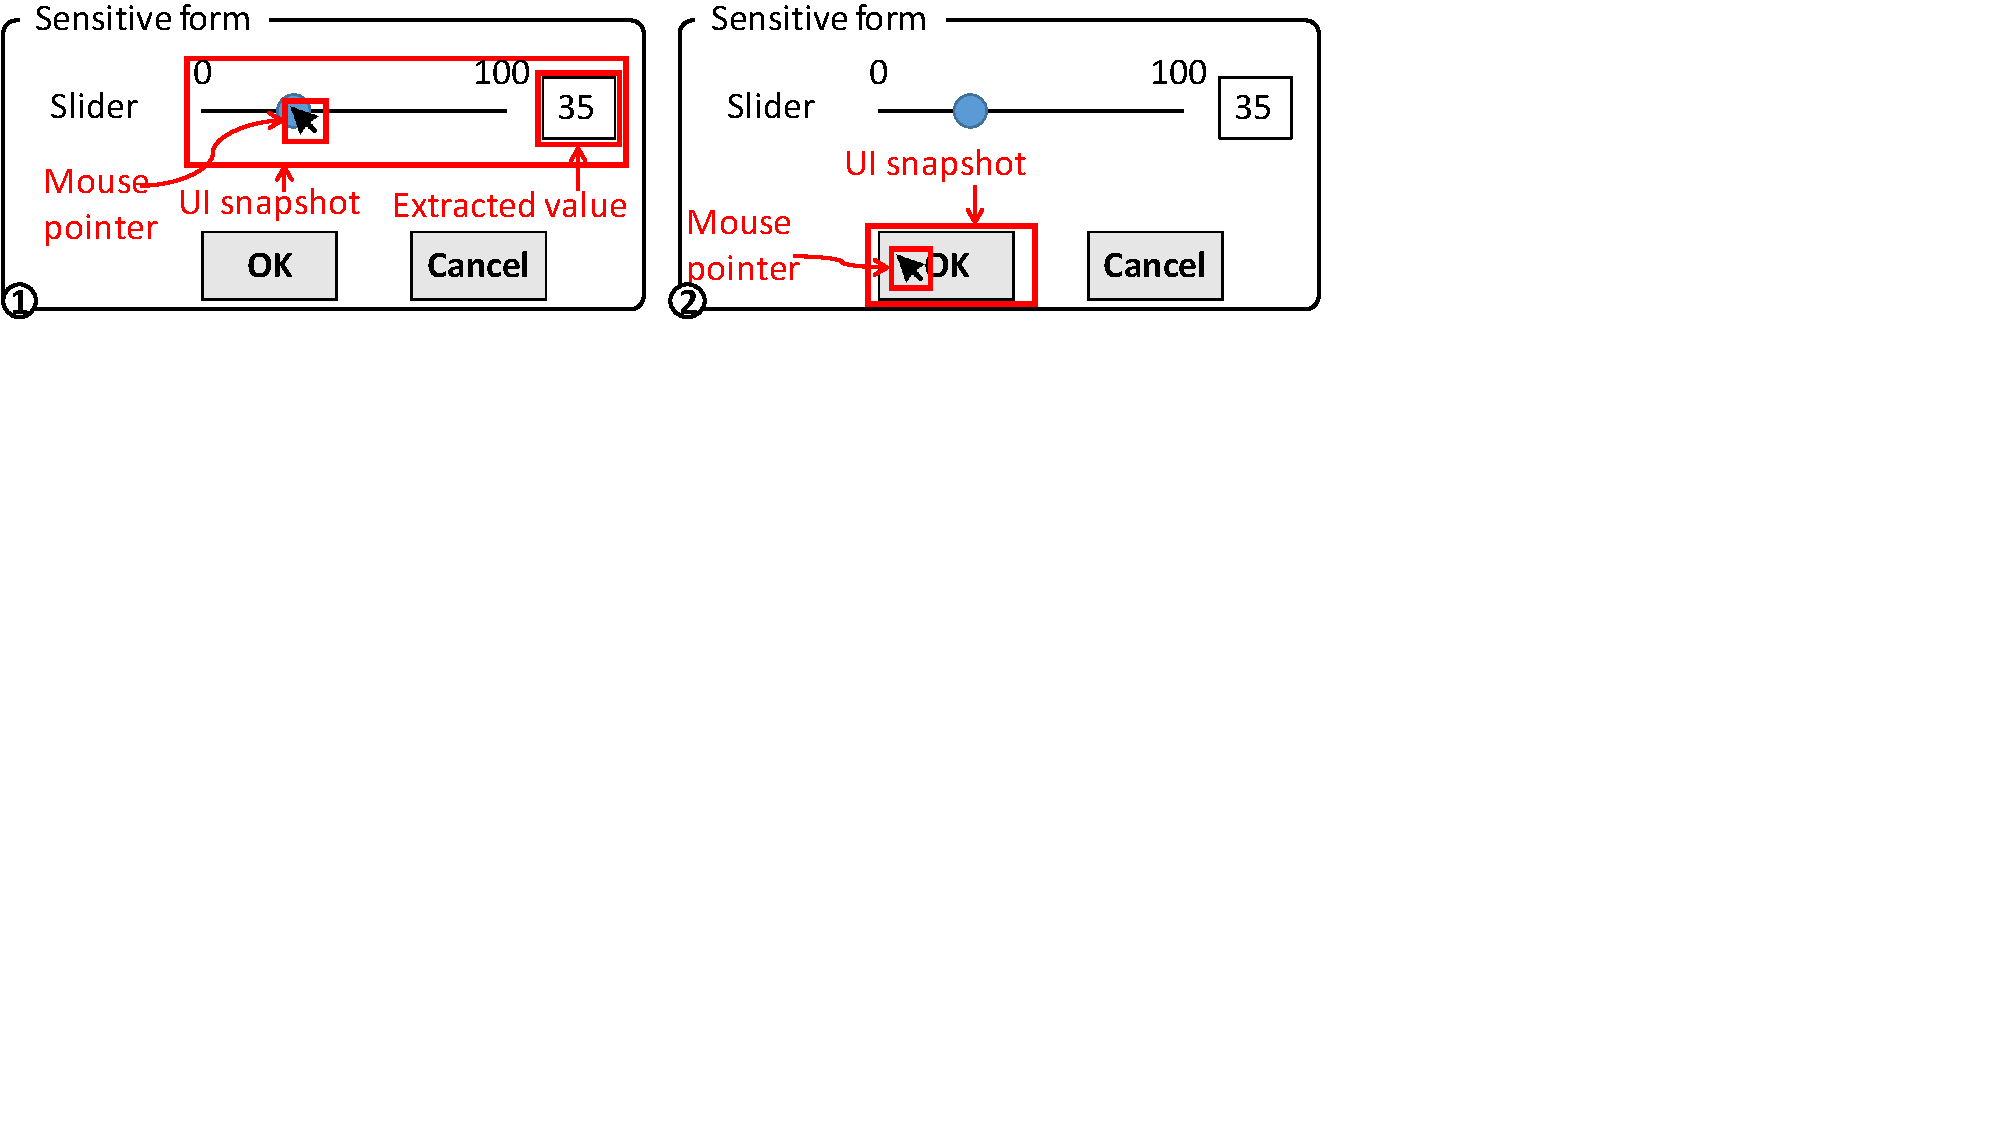
\includegraphics[trim={0 13.5cm 11.5cm 0}, clip, width=\linewidth]{uiDetect_2.pdf}
\caption{\textbf{Strawman solution III: Text/Image Analysis of the UIs}. The external device captures and sends two screenshots to the server. \one when the user sets the slider to the intended position to make sure that the host manipulate the value, and \two the user clicks the \texttt{OK} button to conforms her action.}\spacesave
%\caption{\textbf{Strawman solution III: Text/Image Analysis of the UIs}. This strawman solution uses image/text analysis to detect the UI element leveraging edge detection and optical character recognition (to extract the labels on the UI element). The solution suffers from a lack of robustness where the \device sometime fails to correctly classify the UI elements/labels due to mouse position or colors.}
\label{fig:uiDetect}
\end{figure}
\fi

This strawman solution uses a trusted devices that takes screenshot when the user executes any actione.g., clicking the mouse to submit a form on a webpage. The device then signs the snapshot and transmits it to the server along with the signed input. The signed snapshot by the device could reveal if the untrusted host manipulates the UI. The remote server verifies the signature and then uses image/text analysis to extract the information from the UI elements such as labels on buttons or markers of a slider, etc. However this solution suffers from the following fundamental problems:
%In Figure~\ref{fig:uiDetect} we illustrate an example scenario where the device sends two screenshots of the user interaction \one inputting the value via the slider, and \two confirming the action by pressing the \texttt{OK} button.
%This involves the \device to take a screen-shot from the HDMI frame and use image analysis to understand user action. E.g., in Figure~\ref{fig:uiDetect}, \one the user first drags along the slider UI to set a value (\texttt{35}) and then \two the user clicks on the \texttt{OK}. The \device uses character recognition technique to extract the label and the data from the UI. 
%This example shows the apparent complexity of this mechanism that does not scale with all UI. Further investigation and prototype implementation shows several drawbacks of this solution:
\begin{mylist}
  \item This method does not capture spatiotemporal user context. That implies that the attacker may show some spacial information on the screen to influence user input that may not be captured by the screenshot. The temporal user context implies that taking the snapshot may not capture user intention as for a very short fraction of time the attacker may change the output of the display.
  \item One way to mitigate the previous problem is to capture a video of user interaction. But such as method requires the host to seend a large amount of data to the server and video processing is both time and CPU intensive. 
  \item Adversarial machine learning techniques~\cite{eykholt2017robust,sitawarin2018rogue} could make the image/text recognition technique insecure.
  \item Taking the screenshot also reveal other applications that the user is operating which can be a threat to privacy.
\end{mylist}

%Due to such limitations, and the inherent offline nature of this solution, we developed a more efficient solution to preserve the integrity of user actions on a UI element. We describe the method in the following section. The solution has a trade-off that the developers need to incorporate some small changes to the remote server but provides better security and usability. We describe our solution in the following section.
\fi

\iffalse
\subsection{Challenges}


Modern user interfaces (UIs) are diverse and hard to generalize, resulting in many possible ways to provide input and receiving output.  This makes the protection of IO integrity, and confidentiality is a particularly challenging task. For example, given a mouse movement and clicking on a button from the user, it is necessary to understand the user intention that corresponds to the mouse movements. 


The second challenge arises while ensuring IO confidentiality. For mouse input, hiding the mouse movement while keeping all the regular functionality intact is a challenging task as we do not consider large TCB-based solution such as a trusted hypervisor.


Apart from these functional challenges for implementation, there exist multiple attack vectors that we want to provide protection. 
\fi

\subsection{High-level Description of the System}


\begin{figure}[t]
\centering
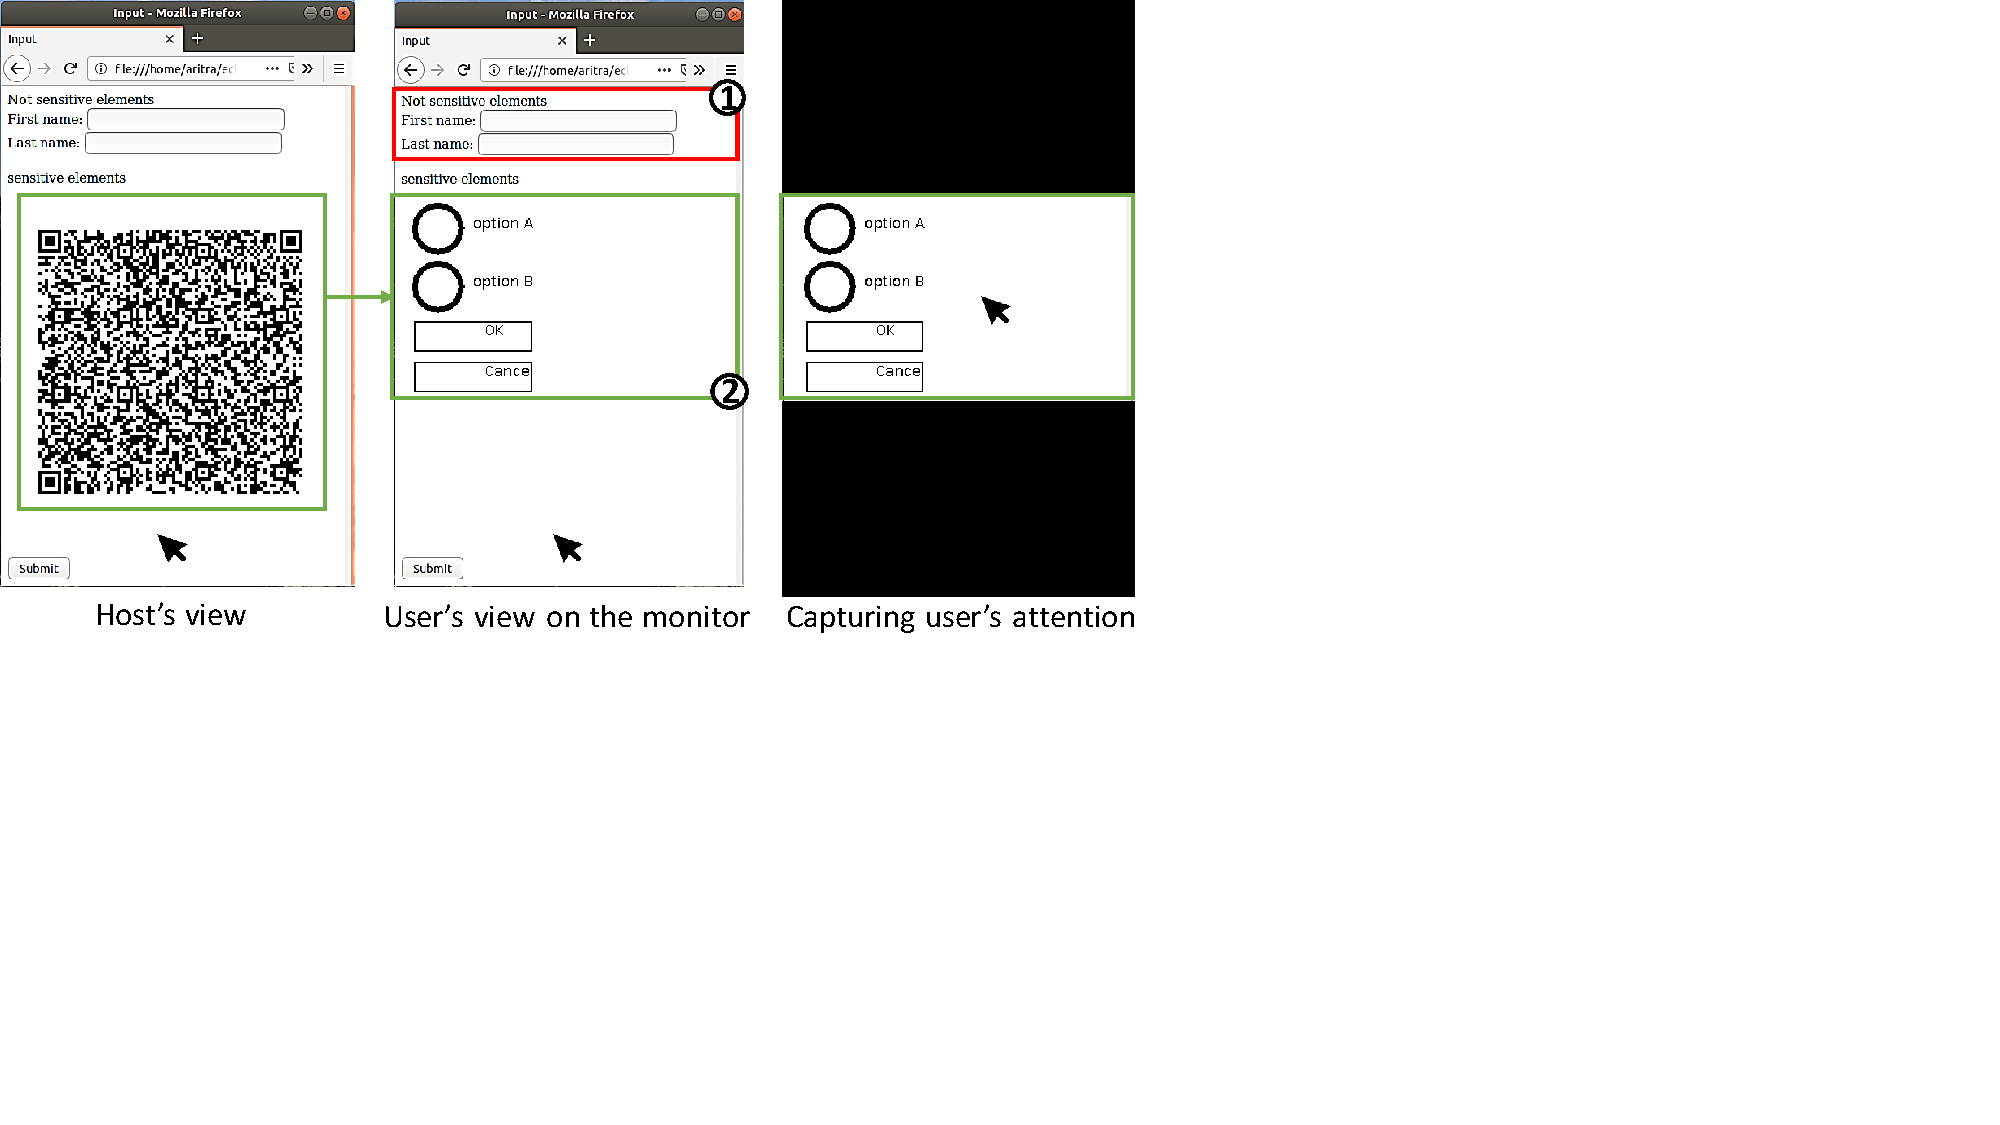
\includegraphics[trim={0 8cm 15cm 0}, clip, width=\linewidth]{overlayScreenShot_new.pdf}
\caption{\textbf{\name high-level approach.} The figure shows the \device overlay of UI elements to protect IO integrity and confidentiality. \one The host only sees the non-protected UI elements and the protect elements are encoded (in our case its the QR code). \two shows the non-protected part of the screen where the UI is rendered by the untrusted host. \three shows the \device generated protected UI overlay that is hidden from the host. The protected part of the screen provides integrity and confidentiality of all user IO. \four shows that the \device dims out rest of the part of the screen when the user moves her mouse pointer over the protected region.}
\spacesave
\label{fig:screenshot_1}
\end{figure}


\myparagraph{Key idea} The drawbacks in the existing and strawman solutions provide the intuition for the design of our solution \name. The key idea of our paper achieve the primary security properties (refer to Section \ref{sec:problemStatement:goals}): i) all the existing trusted path solutions failed to achieve input integrity as both output, and input integrity is needed to be ensured simultaneously to achieve any one of them, and ii) all the input sources are needed to be protected in order to protect any one of them as they can influence each other. \name achieves IO integrity and confidentiality by leveraging a trusted component that we call \device. In our implementation, \device is realized as an external, low-TCB hardware that uses off-the-shelf components and easy to integrate with legacy systems - providing easy \emph{deployment}. 

As seen in Figure~\ref{fig:approachOverview}, \device sits between all IO device and the host system. It intercepts all keyboard and mouse movements, and intercept \& overlay on the display signal. Figure~\ref{fig:screenshot_1} provides a running example of \name where \one the attacker can not observer or manipulate the integrity and confidentiality protected UI that are encoded (the QR code is an example encoding of an encrypted UI in Figure~\ref{fig:screenshot_1}) and signed by the remote server. \two the \device overlays the UI alongside other right UI and \js elements on the screen. Only the \device can interact with the UI elements on the overlay via the connected keyboard and mouse. This way the \device secures i) \emph{both output and input integrity}, and ii) all the \emph{modalities of inputs} that interacts with the protected UI elements.  


\name also reduces the cognitive load from the user by using lightbox mechanism~\cite{huang2012clickjacking}) that is shown in \four. This highlight happens when either the mouse pointer enters the overlaid UI, or the user manually triggers by a sequence of key presses. This allows the user to correctly recognize the overlaid part of the screen. Thus, the untrusted host cannot trick the user to i) follow some instructions that are written by the host, ii) does not leak sensitive data to the host. Note that lightbox is of the many ways to capture the user attention, e.g., freezing the untrusted part of the screen etc. The UI overlay imposes a challenge to \name as \device is oblivious to the actual location of the pointer. To active the user attention mechanisms (such as the lightbox) at the proper time, the \device intercepts all the mouse moves and find the pointer on the screen from the intercepted display signal. The \device draws an overlay of the mouse pointer on to of the host mouse pointer so that the user can follow the legitimate mouse pointer easily. This way, the \device ensure that the user and the \device is tracking the same mouse pointer on the screen. 
%In summary, \name could be used in two ways, i) only integrity where the IO integrity is protected. E.g., remote safety-critical devices require IO integrity for their safe operations, and ii) both integrity and confidentiality, e.g., financial transactions where the user credentials are needed to be hidden from the untrusted host.
%Note that \name's way of highlighting the overlaid elements on the screen is more effective in focusing user's attention on the sensitive UI elements. 
%Note, that \name's way of isolating the overlaid UI and focusing user attention to it does not require any training to use the system.


%As shown in Figure~\ref{fig:screenshot_1}, \name provides output integrity by overlaying the sensitive UI elements on the screen that is sent directly from the trusted remote server in an encoded format (the QR code is an example encoding of an encrypted UI in Figure~\ref{fig:screenshot_1}). The remote server signs the overlaid UI that the \device verifies before overlay. Hence, sensitive UI elements cannot be modified by the untrusted host. By only overlaying on a limited part of the screen, \name does not require to change the layout of a complex, content-heavy webpage as rest of the part of the screen could be left unmodified.

%Moreover, the secure part of the screen, i.e., the overlay can support complex UI and user interactions that are common in today's web. All the interactions on this overlaid UI are intercepted, signed, and sent to the remote server by the \device. Thus \name ensures input integrity and confidentiality. As only the user can interact with the overlaid UI, the host cannot see the content of the UI, user's input, or trigger early submission of the data.
%\name minimizes the cognitive load on the user by highlighting and dimming out untrusted part of the screen (the method is known as the lighbox~\cite{huang2012clickjacking}) that is shown in Figure~\ref{fig:screenshot_1}. This highlight happens when either the mouse pointer enters the overlaid UI, or the user manually triggers by a sequence of key presses. This allows the user to correctly recognize the overlaid part of the screen. Thus, the untrusted host cannot trick the user to i) follow some instructions that are written by the host, ii) does not leak sensitive data to the host. Note that \name's way of highlighting the overlaid elements on the screen is more effective in focusing user's attention on the sensitive UI elements. Note, that \name's way of isolating the overlaid UI and focusing user attention to it does not require any training to use the system. Hence, the integrity property of \name can be achieved out of the box. However, for confidentiality, it is mandatory that the user engages the focusing activity manually to determine the overlaid UI to avoid revealing her sensitive data to the host. The notion of increasing security by some simple user activity is very common in day to day's system such as opening incognito mode in the browser to avoid tracking information.
%To prevent clickjacking attacks, \device intercepts all the mouse moves and find the pointer on the screen from the intercepted display signal. This allows the \device to maintain pointer integrity where the \device can check if all the mouse pointer activities on the screen are executed by the user. The \device also draws an overlay of the mouse pointer on to of the host mouse pointer so that the user can follow the legitimate mouse pointer easily. In summary, \name could be used in two ways, i) only integrity where the IO integrity is protected. E.g., remote safety-critical devices require IO integrity for their safe operations, and ii) both integrity and confidentiality, e.g., financial transactions where the user credentials are needed to be hidden from the untrusted host.  


%%%%%%%%%%%%%%%%%%%%%%%%%%%%%%%%%%%%%%%%%%%%%%%%%%%%%%%%%%%%%%
%%OLD text

% \myparagraph{Key idea} The strawman solutions in the previous section ((see Section~\ref{sec:approach:strawman})) provides the intuition for the design of our solution \name. All the exiting trusted path solution failed to achieve input integrity as both output and input integrity is needed to maintain simultaneously in order to achieve anyone of them.
% 
% The goal of the \device is to guarantee the security %the integrity (and the confidentiality when required) 
% of the user interaction with a sensitive application on the remote server. Our system configuration provides the \device with two capabilities: i) intercept the raw inputs generated by the user, and ii) render UI objects on the HDMI frame that is displayed on the screen. 
% The first capability guarantees that the user inputs arrive directly to a trusted component (\device); therefore, the compromised host cannot manipulate them. However, as described in the strawman solution I (see Section~\ref{sec:approach:strawman}) this functionality alone cannot assure the security of the user inputs. The second capability allows the \device to render trusted objects on the screen such as input elements, or data sent from the remote server. 
% 
% To achieve its goal, the \device initially ensures the integrity of the output from the remote server, i.e., makes sure to present the right context to the user. Considering that the code size running on the \device is small, it renders only simple UI objects for sensitive elements, while the remaining UI is still generated by the host as illustrated in Figure~\ref{fig:screenshot_1}. The \device tracks continuously the cursor to understand correctly user's intentions (e.g., submit a form, or cancel a transaction). On top of the host's cursor, the \device renders its image of the cursor which is more prominent and ensures that the user and the \device follow the same cursor to prevent clickjacking. Additionally, the \device highlights the legitimate cursor on specific events to guarantee that the user follows the same cursor, which in the same time also exposes any attempt of the malicious host to trick the user by creating a fake cursor. %Also, user inputs addressed to the sensitive elements are managed by the device and rendered on runtime as overlays in HDMI frames to provide feedback to the user. 
% 
% During the initialization phase, the \device and the remote server share a key that is used to encrypt/sign (depends on the application if IO confidentiality is required) the communication between each other. Note that the \device does not have any network capabilities, instead uses the host as an untrusted transport. The remote server signs the sensitive elements that should be protected and delivers them to the untrusted host. The application running on the host encodes the sensitive elements into the HDMI frame. The \device captures the frames, decodes the sensitive elements, verifies their signatures, and then renders elements into an overlay. Figure~\ref{fig:screenshot_1} provides a screenshot of the attacker's view of the screen and the user's view after the \device overlays the UI. \one shows non-sensitive elements that are unprotected, while \two are the protected elements that are rendered by the \device. In this way, the device guarantees that the user is presented with the legitimate elements sent by the remote server and the user interaction with these elements is managed only by the device.
%   
% User inputs (mouse events and keystrokes) addressed to the protected elements are intercepted by the \device and not forwarded to the untrusted host. The \device renders on runtime the user inputs into the overlay while the host is oblivious about them. From the user's perspective, the workflow of filling a form with protected elements remains the same as filling forms of existing applications. However, when the user interacts with regular applications that do not require \name protection, the \device operates in a \texttt{light} mode. The \device mostly serves as a relaying device that forwards mouse and keyboard inputs to the host and HDMI frames from the host to the display. Hence, the user experience is not affected when interacting with other applications. 


